%-*-latex-*-
\tinysidebar{\debug{exercises/{introduction-to-group-theory-0/answer.tex}}}
To check if $C_2$ is abelian, I need to check that
\[
x * y = y * x
\]
for all $x, y \in G$.
Here are checks for all the cases for $C_2$:
\begin{align*}
e * e &= e = e * e \\
e * a &= a = a * e \\
a * e &= a = e * a \\
a * a &= e = a * a
\end{align*}
Therefore $C_2$ is abelian.

It should be clear that you need not check
\[
x * y = y * x
\]
for \textit{all} $x, y \in G$.
Using an example, the only cases that need to be checked are the
entries marked X for this group table:
%-*-latex-*-
\begin{center}
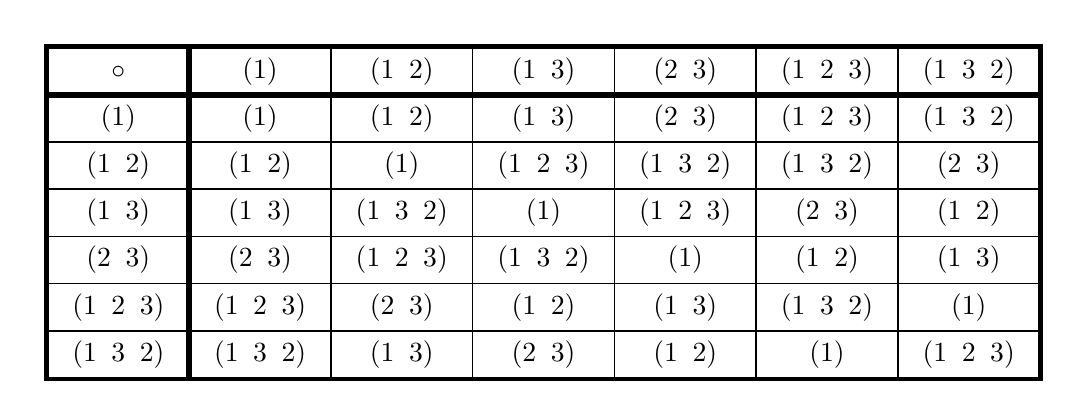
\begin{tikzpicture}

\draw (0.9, -0.3)
  node[draw, line width=0.02cm, , color=black,
       rounded corners=0cm, inner sep=0cm] {

\begin{minipage}[t][0.6cm]{1.8cm}
\mbox{}

\end{minipage}

};\draw (0.9, -0.3) node[color=black] {{\texttt{{\vphantom{$\circ$$(1)$$(1 \ 2)$$(1 \ 3)$$(2 \ 3)$$(1 \ 2 \ 3)$$(1 \ 3 \ 2)$}$\circ$}}}};\node[anchor=south] at (0.9,0.01) {};\node[anchor=east] at (-0.01,-0.3) {};
\draw (0.9, -0.3)
  node[draw, line width=0.06cm, , color=black,
       rounded corners=0cm, inner sep=0cm] {

\begin{minipage}[t][0.62cm]{1.82cm}
\mbox{}

\end{minipage}

};
\draw (2.7, -0.3)
  node[draw, line width=0.02cm, , color=black,
       rounded corners=0cm, inner sep=0cm] {

\begin{minipage}[t][0.6cm]{1.8cm}
\mbox{}

\end{minipage}

};\draw (2.7, -0.3) node[color=black] {{\texttt{{\vphantom{$\circ$$(1)$$(1 \ 2)$$(1 \ 3)$$(2 \ 3)$$(1 \ 2 \ 3)$$(1 \ 3 \ 2)$}$(1)$}}}};
\draw (4.5, -0.3)
  node[draw, line width=0.02cm, , color=black,
       rounded corners=0cm, inner sep=0cm] {

\begin{minipage}[t][0.6cm]{1.8cm}
\mbox{}

\end{minipage}

};\draw (4.5, -0.3) node[color=black] {{\texttt{{\vphantom{$\circ$$(1)$$(1 \ 2)$$(1 \ 3)$$(2 \ 3)$$(1 \ 2 \ 3)$$(1 \ 3 \ 2)$}$(1 \ 2)$}}}};
\draw (6.300000000000001, -0.3)
  node[draw, line width=0.02cm, , color=black,
       rounded corners=0cm, inner sep=0cm] {

\begin{minipage}[t][0.6cm]{1.8cm}
\mbox{}

\end{minipage}

};\draw (6.300000000000001, -0.3) node[color=black] {{\texttt{{\vphantom{$\circ$$(1)$$(1 \ 2)$$(1 \ 3)$$(2 \ 3)$$(1 \ 2 \ 3)$$(1 \ 3 \ 2)$}$(1 \ 3)$}}}};
\draw (8.100000000000001, -0.3)
  node[draw, line width=0.02cm, , color=black,
       rounded corners=0cm, inner sep=0cm] {

\begin{minipage}[t][0.6cm]{1.8cm}
\mbox{}

\end{minipage}

};\draw (8.100000000000001, -0.3) node[color=black] {{\texttt{{\vphantom{$\circ$$(1)$$(1 \ 2)$$(1 \ 3)$$(2 \ 3)$$(1 \ 2 \ 3)$$(1 \ 3 \ 2)$}$(2 \ 3)$}}}};
\draw (9.9, -0.3)
  node[draw, line width=0.02cm, , color=black,
       rounded corners=0cm, inner sep=0cm] {

\begin{minipage}[t][0.6cm]{1.8cm}
\mbox{}

\end{minipage}

};\draw (9.9, -0.3) node[color=black] {{\texttt{{\vphantom{$\circ$$(1)$$(1 \ 2)$$(1 \ 3)$$(2 \ 3)$$(1 \ 2 \ 3)$$(1 \ 3 \ 2)$}$(1 \ 2 \ 3)$}}}};
\draw (11.700000000000001, -0.3)
  node[draw, line width=0.02cm, , color=black,
       rounded corners=0cm, inner sep=0cm] {

\begin{minipage}[t][0.6cm]{1.8cm}
\mbox{}

\end{minipage}

};\draw (11.700000000000001, -0.3) node[color=black] {{\texttt{{\vphantom{$\circ$$(1)$$(1 \ 2)$$(1 \ 3)$$(2 \ 3)$$(1 \ 2 \ 3)$$(1 \ 3 \ 2)$}$(1 \ 3 \ 2)$}}}};\node[anchor=south] at (2.7,0.01) {};\node[anchor=south] at (4.5,0.01) {};\node[anchor=south] at (6.300000000000001,0.01) {};\node[anchor=south] at (8.100000000000001,0.01) {};\node[anchor=south] at (9.9,0.01) {};\node[anchor=south] at (11.700000000000001,0.01) {};\node[anchor=east] at (1.79,-0.3) {};
\draw (7.2, -0.3)
  node[draw, line width=0.06cm, , color=black,
       rounded corners=0cm, inner sep=0cm] {

\begin{minipage}[t][0.62cm]{10.82cm}
\mbox{}

\end{minipage}

};
\draw (0.9, -0.8999999999999999)
  node[draw, line width=0.02cm, , color=black,
       rounded corners=0cm, inner sep=0cm] {

\begin{minipage}[t][0.6cm]{1.8cm}
\mbox{}

\end{minipage}

};\draw (0.9, -0.8999999999999999) node[color=black] {{\texttt{{\vphantom{$\circ$$(1)$$(1 \ 2)$$(1 \ 3)$$(2 \ 3)$$(1 \ 2 \ 3)$$(1 \ 3 \ 2)$}$(1)$}}}};
\draw (0.9, -1.4999999999999998)
  node[draw, line width=0.02cm, , color=black,
       rounded corners=0cm, inner sep=0cm] {

\begin{minipage}[t][0.6cm]{1.8cm}
\mbox{}

\end{minipage}

};\draw (0.9, -1.4999999999999998) node[color=black] {{\texttt{{\vphantom{$\circ$$(1)$$(1 \ 2)$$(1 \ 3)$$(2 \ 3)$$(1 \ 2 \ 3)$$(1 \ 3 \ 2)$}$(1 \ 2)$}}}};
\draw (0.9, -2.0999999999999996)
  node[draw, line width=0.02cm, , color=black,
       rounded corners=0cm, inner sep=0cm] {

\begin{minipage}[t][0.6cm]{1.8cm}
\mbox{}

\end{minipage}

};\draw (0.9, -2.0999999999999996) node[color=black] {{\texttt{{\vphantom{$\circ$$(1)$$(1 \ 2)$$(1 \ 3)$$(2 \ 3)$$(1 \ 2 \ 3)$$(1 \ 3 \ 2)$}$(1 \ 3)$}}}};
\draw (0.9, -2.7)
  node[draw, line width=0.02cm, , color=black,
       rounded corners=0cm, inner sep=0cm] {

\begin{minipage}[t][0.6cm]{1.8cm}
\mbox{}

\end{minipage}

};\draw (0.9, -2.7) node[color=black] {{\texttt{{\vphantom{$\circ$$(1)$$(1 \ 2)$$(1 \ 3)$$(2 \ 3)$$(1 \ 2 \ 3)$$(1 \ 3 \ 2)$}$(2 \ 3)$}}}};
\draw (0.9, -3.3000000000000007)
  node[draw, line width=0.02cm, , color=black,
       rounded corners=0cm, inner sep=0cm] {

\begin{minipage}[t][0.6cm]{1.8cm}
\mbox{}

\end{minipage}

};\draw (0.9, -3.3000000000000007) node[color=black] {{\texttt{{\vphantom{$\circ$$(1)$$(1 \ 2)$$(1 \ 3)$$(2 \ 3)$$(1 \ 2 \ 3)$$(1 \ 3 \ 2)$}$(1 \ 2 \ 3)$}}}};
\draw (0.9, -3.9000000000000004)
  node[draw, line width=0.02cm, , color=black,
       rounded corners=0cm, inner sep=0cm] {

\begin{minipage}[t][0.6cm]{1.8cm}
\mbox{}

\end{minipage}

};\draw (0.9, -3.9000000000000004) node[color=black] {{\texttt{{\vphantom{$\circ$$(1)$$(1 \ 2)$$(1 \ 3)$$(2 \ 3)$$(1 \ 2 \ 3)$$(1 \ 3 \ 2)$}$(1 \ 3 \ 2)$}}}};\node[anchor=south] at (0.9,-0.59) {};\node[anchor=east] at (-0.01,-0.8999999999999999) {};\node[anchor=east] at (-0.01,-1.4999999999999998) {};\node[anchor=east] at (-0.01,-2.0999999999999996) {};\node[anchor=east] at (-0.01,-2.7) {};\node[anchor=east] at (-0.01,-3.3000000000000007) {};\node[anchor=east] at (-0.01,-3.9000000000000004) {};
\draw (0.9, -2.4)
  node[draw, line width=0.06cm, , color=black,
       rounded corners=0cm, inner sep=0cm] {

\begin{minipage}[t][3.62cm]{1.82cm}
\mbox{}

\end{minipage}

};
\draw (2.7, -0.8999999999999999)
  node[draw, line width=0.02cm, , color=black,
       rounded corners=0cm, inner sep=0cm] {

\begin{minipage}[t][0.6cm]{1.8cm}
\mbox{}

\end{minipage}

};\draw (2.7, -0.8999999999999999) node[color=black] {{\texttt{{\vphantom{$\circ$$(1)$$(1 \ 2)$$(1 \ 3)$$(2 \ 3)$$(1 \ 2 \ 3)$$(1 \ 3 \ 2)$}$(1)$}}}};
\draw (4.5, -0.8999999999999999)
  node[draw, line width=0.02cm, , color=black,
       rounded corners=0cm, inner sep=0cm] {

\begin{minipage}[t][0.6cm]{1.8cm}
\mbox{}

\end{minipage}

};\draw (4.5, -0.8999999999999999) node[color=black] {{\texttt{{\vphantom{$\circ$$(1)$$(1 \ 2)$$(1 \ 3)$$(2 \ 3)$$(1 \ 2 \ 3)$$(1 \ 3 \ 2)$}$(1 \ 2)$}}}};
\draw (6.300000000000001, -0.8999999999999999)
  node[draw, line width=0.02cm, , color=black,
       rounded corners=0cm, inner sep=0cm] {

\begin{minipage}[t][0.6cm]{1.8cm}
\mbox{}

\end{minipage}

};\draw (6.300000000000001, -0.8999999999999999) node[color=black] {{\texttt{{\vphantom{$\circ$$(1)$$(1 \ 2)$$(1 \ 3)$$(2 \ 3)$$(1 \ 2 \ 3)$$(1 \ 3 \ 2)$}$(1 \ 3)$}}}};
\draw (8.100000000000001, -0.8999999999999999)
  node[draw, line width=0.02cm, , color=black,
       rounded corners=0cm, inner sep=0cm] {

\begin{minipage}[t][0.6cm]{1.8cm}
\mbox{}

\end{minipage}

};\draw (8.100000000000001, -0.8999999999999999) node[color=black] {{\texttt{{\vphantom{$\circ$$(1)$$(1 \ 2)$$(1 \ 3)$$(2 \ 3)$$(1 \ 2 \ 3)$$(1 \ 3 \ 2)$}$(2 \ 3)$}}}};
\draw (9.9, -0.8999999999999999)
  node[draw, line width=0.02cm, , color=black,
       rounded corners=0cm, inner sep=0cm] {

\begin{minipage}[t][0.6cm]{1.8cm}
\mbox{}

\end{minipage}

};\draw (9.9, -0.8999999999999999) node[color=black] {{\texttt{{\vphantom{$\circ$$(1)$$(1 \ 2)$$(1 \ 3)$$(2 \ 3)$$(1 \ 2 \ 3)$$(1 \ 3 \ 2)$}$(1 \ 2 \ 3)$}}}};
\draw (11.700000000000001, -0.8999999999999999)
  node[draw, line width=0.02cm, , color=black,
       rounded corners=0cm, inner sep=0cm] {

\begin{minipage}[t][0.6cm]{1.8cm}
\mbox{}

\end{minipage}

};\draw (11.700000000000001, -0.8999999999999999) node[color=black] {{\texttt{{\vphantom{$\circ$$(1)$$(1 \ 2)$$(1 \ 3)$$(2 \ 3)$$(1 \ 2 \ 3)$$(1 \ 3 \ 2)$}$(1 \ 3 \ 2)$}}}};
\draw (2.7, -1.4999999999999998)
  node[draw, line width=0.02cm, , color=black,
       rounded corners=0cm, inner sep=0cm] {

\begin{minipage}[t][0.6cm]{1.8cm}
\mbox{}

\end{minipage}

};\draw (2.7, -1.4999999999999998) node[color=black] {{\texttt{{\vphantom{$\circ$$(1)$$(1 \ 2)$$(1 \ 3)$$(2 \ 3)$$(1 \ 2 \ 3)$$(1 \ 3 \ 2)$}$(1 \ 2)$}}}};
\draw (4.5, -1.4999999999999998)
  node[draw, line width=0.02cm, , color=black,
       rounded corners=0cm, inner sep=0cm] {

\begin{minipage}[t][0.6cm]{1.8cm}
\mbox{}

\end{minipage}

};\draw (4.5, -1.4999999999999998) node[color=black] {{\texttt{{\vphantom{$\circ$$(1)$$(1 \ 2)$$(1 \ 3)$$(2 \ 3)$$(1 \ 2 \ 3)$$(1 \ 3 \ 2)$}$(1)$}}}};
\draw (6.300000000000001, -1.4999999999999998)
  node[draw, line width=0.02cm, , color=black,
       rounded corners=0cm, inner sep=0cm] {

\begin{minipage}[t][0.6cm]{1.8cm}
\mbox{}

\end{minipage}

};\draw (6.300000000000001, -1.4999999999999998) node[color=black] {{\texttt{{\vphantom{$\circ$$(1)$$(1 \ 2)$$(1 \ 3)$$(2 \ 3)$$(1 \ 2 \ 3)$$(1 \ 3 \ 2)$}$(1 \ 2 \ 3)$}}}};
\draw (8.100000000000001, -1.4999999999999998)
  node[draw, line width=0.02cm, , color=black,
       rounded corners=0cm, inner sep=0cm] {

\begin{minipage}[t][0.6cm]{1.8cm}
\mbox{}

\end{minipage}

};\draw (8.100000000000001, -1.4999999999999998) node[color=black] {{\texttt{{\vphantom{$\circ$$(1)$$(1 \ 2)$$(1 \ 3)$$(2 \ 3)$$(1 \ 2 \ 3)$$(1 \ 3 \ 2)$}$(1 \ 3 \ 2)$}}}};
\draw (9.9, -1.4999999999999998)
  node[draw, line width=0.02cm, , color=black,
       rounded corners=0cm, inner sep=0cm] {

\begin{minipage}[t][0.6cm]{1.8cm}
\mbox{}

\end{minipage}

};\draw (9.9, -1.4999999999999998) node[color=black] {{\texttt{{\vphantom{$\circ$$(1)$$(1 \ 2)$$(1 \ 3)$$(2 \ 3)$$(1 \ 2 \ 3)$$(1 \ 3 \ 2)$}$(1 \ 3 \ 2)$}}}};
\draw (11.700000000000001, -1.4999999999999998)
  node[draw, line width=0.02cm, , color=black,
       rounded corners=0cm, inner sep=0cm] {

\begin{minipage}[t][0.6cm]{1.8cm}
\mbox{}

\end{minipage}

};\draw (11.700000000000001, -1.4999999999999998) node[color=black] {{\texttt{{\vphantom{$\circ$$(1)$$(1 \ 2)$$(1 \ 3)$$(2 \ 3)$$(1 \ 2 \ 3)$$(1 \ 3 \ 2)$}$(2 \ 3)$}}}};
\draw (2.7, -2.0999999999999996)
  node[draw, line width=0.02cm, , color=black,
       rounded corners=0cm, inner sep=0cm] {

\begin{minipage}[t][0.6cm]{1.8cm}
\mbox{}

\end{minipage}

};\draw (2.7, -2.0999999999999996) node[color=black] {{\texttt{{\vphantom{$\circ$$(1)$$(1 \ 2)$$(1 \ 3)$$(2 \ 3)$$(1 \ 2 \ 3)$$(1 \ 3 \ 2)$}$(1 \ 3)$}}}};
\draw (4.5, -2.0999999999999996)
  node[draw, line width=0.02cm, , color=black,
       rounded corners=0cm, inner sep=0cm] {

\begin{minipage}[t][0.6cm]{1.8cm}
\mbox{}

\end{minipage}

};\draw (4.5, -2.0999999999999996) node[color=black] {{\texttt{{\vphantom{$\circ$$(1)$$(1 \ 2)$$(1 \ 3)$$(2 \ 3)$$(1 \ 2 \ 3)$$(1 \ 3 \ 2)$}$(1 \ 3 \ 2)$}}}};
\draw (6.300000000000001, -2.0999999999999996)
  node[draw, line width=0.02cm, , color=black,
       rounded corners=0cm, inner sep=0cm] {

\begin{minipage}[t][0.6cm]{1.8cm}
\mbox{}

\end{minipage}

};\draw (6.300000000000001, -2.0999999999999996) node[color=black] {{\texttt{{\vphantom{$\circ$$(1)$$(1 \ 2)$$(1 \ 3)$$(2 \ 3)$$(1 \ 2 \ 3)$$(1 \ 3 \ 2)$}$(1)$}}}};
\draw (8.100000000000001, -2.0999999999999996)
  node[draw, line width=0.02cm, , color=black,
       rounded corners=0cm, inner sep=0cm] {

\begin{minipage}[t][0.6cm]{1.8cm}
\mbox{}

\end{minipage}

};\draw (8.100000000000001, -2.0999999999999996) node[color=black] {{\texttt{{\vphantom{$\circ$$(1)$$(1 \ 2)$$(1 \ 3)$$(2 \ 3)$$(1 \ 2 \ 3)$$(1 \ 3 \ 2)$}$(1 \ 2 \ 3)$}}}};
\draw (9.9, -2.0999999999999996)
  node[draw, line width=0.02cm, , color=black,
       rounded corners=0cm, inner sep=0cm] {

\begin{minipage}[t][0.6cm]{1.8cm}
\mbox{}

\end{minipage}

};\draw (9.9, -2.0999999999999996) node[color=black] {{\texttt{{\vphantom{$\circ$$(1)$$(1 \ 2)$$(1 \ 3)$$(2 \ 3)$$(1 \ 2 \ 3)$$(1 \ 3 \ 2)$}$(2 \ 3)$}}}};
\draw (11.700000000000001, -2.0999999999999996)
  node[draw, line width=0.02cm, , color=black,
       rounded corners=0cm, inner sep=0cm] {

\begin{minipage}[t][0.6cm]{1.8cm}
\mbox{}

\end{minipage}

};\draw (11.700000000000001, -2.0999999999999996) node[color=black] {{\texttt{{\vphantom{$\circ$$(1)$$(1 \ 2)$$(1 \ 3)$$(2 \ 3)$$(1 \ 2 \ 3)$$(1 \ 3 \ 2)$}$(1 \ 2)$}}}};
\draw (2.7, -2.7)
  node[draw, line width=0.02cm, , color=black,
       rounded corners=0cm, inner sep=0cm] {

\begin{minipage}[t][0.6cm]{1.8cm}
\mbox{}

\end{minipage}

};\draw (2.7, -2.7) node[color=black] {{\texttt{{\vphantom{$\circ$$(1)$$(1 \ 2)$$(1 \ 3)$$(2 \ 3)$$(1 \ 2 \ 3)$$(1 \ 3 \ 2)$}$(2 \ 3)$}}}};
\draw (4.5, -2.7)
  node[draw, line width=0.02cm, , color=black,
       rounded corners=0cm, inner sep=0cm] {

\begin{minipage}[t][0.6cm]{1.8cm}
\mbox{}

\end{minipage}

};\draw (4.5, -2.7) node[color=black] {{\texttt{{\vphantom{$\circ$$(1)$$(1 \ 2)$$(1 \ 3)$$(2 \ 3)$$(1 \ 2 \ 3)$$(1 \ 3 \ 2)$}$(1 \ 2 \ 3)$}}}};
\draw (6.300000000000001, -2.7)
  node[draw, line width=0.02cm, , color=black,
       rounded corners=0cm, inner sep=0cm] {

\begin{minipage}[t][0.6cm]{1.8cm}
\mbox{}

\end{minipage}

};\draw (6.300000000000001, -2.7) node[color=black] {{\texttt{{\vphantom{$\circ$$(1)$$(1 \ 2)$$(1 \ 3)$$(2 \ 3)$$(1 \ 2 \ 3)$$(1 \ 3 \ 2)$}$(1 \ 3 \ 2)$}}}};
\draw (8.100000000000001, -2.7)
  node[draw, line width=0.02cm, , color=black,
       rounded corners=0cm, inner sep=0cm] {

\begin{minipage}[t][0.6cm]{1.8cm}
\mbox{}

\end{minipage}

};\draw (8.100000000000001, -2.7) node[color=black] {{\texttt{{\vphantom{$\circ$$(1)$$(1 \ 2)$$(1 \ 3)$$(2 \ 3)$$(1 \ 2 \ 3)$$(1 \ 3 \ 2)$}$(1)$}}}};
\draw (9.9, -2.7)
  node[draw, line width=0.02cm, , color=black,
       rounded corners=0cm, inner sep=0cm] {

\begin{minipage}[t][0.6cm]{1.8cm}
\mbox{}

\end{minipage}

};\draw (9.9, -2.7) node[color=black] {{\texttt{{\vphantom{$\circ$$(1)$$(1 \ 2)$$(1 \ 3)$$(2 \ 3)$$(1 \ 2 \ 3)$$(1 \ 3 \ 2)$}$(1 \ 2)$}}}};
\draw (11.700000000000001, -2.7)
  node[draw, line width=0.02cm, , color=black,
       rounded corners=0cm, inner sep=0cm] {

\begin{minipage}[t][0.6cm]{1.8cm}
\mbox{}

\end{minipage}

};\draw (11.700000000000001, -2.7) node[color=black] {{\texttt{{\vphantom{$\circ$$(1)$$(1 \ 2)$$(1 \ 3)$$(2 \ 3)$$(1 \ 2 \ 3)$$(1 \ 3 \ 2)$}$(1 \ 3)$}}}};
\draw (2.7, -3.3000000000000007)
  node[draw, line width=0.02cm, , color=black,
       rounded corners=0cm, inner sep=0cm] {

\begin{minipage}[t][0.6cm]{1.8cm}
\mbox{}

\end{minipage}

};\draw (2.7, -3.3000000000000007) node[color=black] {{\texttt{{\vphantom{$\circ$$(1)$$(1 \ 2)$$(1 \ 3)$$(2 \ 3)$$(1 \ 2 \ 3)$$(1 \ 3 \ 2)$}$(1 \ 2 \ 3)$}}}};
\draw (4.5, -3.3000000000000007)
  node[draw, line width=0.02cm, , color=black,
       rounded corners=0cm, inner sep=0cm] {

\begin{minipage}[t][0.6cm]{1.8cm}
\mbox{}

\end{minipage}

};\draw (4.5, -3.3000000000000007) node[color=black] {{\texttt{{\vphantom{$\circ$$(1)$$(1 \ 2)$$(1 \ 3)$$(2 \ 3)$$(1 \ 2 \ 3)$$(1 \ 3 \ 2)$}$(2 \ 3)$}}}};
\draw (6.300000000000001, -3.3000000000000007)
  node[draw, line width=0.02cm, , color=black,
       rounded corners=0cm, inner sep=0cm] {

\begin{minipage}[t][0.6cm]{1.8cm}
\mbox{}

\end{minipage}

};\draw (6.300000000000001, -3.3000000000000007) node[color=black] {{\texttt{{\vphantom{$\circ$$(1)$$(1 \ 2)$$(1 \ 3)$$(2 \ 3)$$(1 \ 2 \ 3)$$(1 \ 3 \ 2)$}$(1 \ 2)$}}}};
\draw (8.100000000000001, -3.3000000000000007)
  node[draw, line width=0.02cm, , color=black,
       rounded corners=0cm, inner sep=0cm] {

\begin{minipage}[t][0.6cm]{1.8cm}
\mbox{}

\end{minipage}

};\draw (8.100000000000001, -3.3000000000000007) node[color=black] {{\texttt{{\vphantom{$\circ$$(1)$$(1 \ 2)$$(1 \ 3)$$(2 \ 3)$$(1 \ 2 \ 3)$$(1 \ 3 \ 2)$}$(1 \ 3)$}}}};
\draw (9.9, -3.3000000000000007)
  node[draw, line width=0.02cm, , color=black,
       rounded corners=0cm, inner sep=0cm] {

\begin{minipage}[t][0.6cm]{1.8cm}
\mbox{}

\end{minipage}

};\draw (9.9, -3.3000000000000007) node[color=black] {{\texttt{{\vphantom{$\circ$$(1)$$(1 \ 2)$$(1 \ 3)$$(2 \ 3)$$(1 \ 2 \ 3)$$(1 \ 3 \ 2)$}$(1 \ 3 \ 2)$}}}};
\draw (11.700000000000001, -3.3000000000000007)
  node[draw, line width=0.02cm, , color=black,
       rounded corners=0cm, inner sep=0cm] {

\begin{minipage}[t][0.6cm]{1.8cm}
\mbox{}

\end{minipage}

};\draw (11.700000000000001, -3.3000000000000007) node[color=black] {{\texttt{{\vphantom{$\circ$$(1)$$(1 \ 2)$$(1 \ 3)$$(2 \ 3)$$(1 \ 2 \ 3)$$(1 \ 3 \ 2)$}$(1)$}}}};
\draw (2.7, -3.9000000000000004)
  node[draw, line width=0.02cm, , color=black,
       rounded corners=0cm, inner sep=0cm] {

\begin{minipage}[t][0.6cm]{1.8cm}
\mbox{}

\end{minipage}

};\draw (2.7, -3.9000000000000004) node[color=black] {{\texttt{{\vphantom{$\circ$$(1)$$(1 \ 2)$$(1 \ 3)$$(2 \ 3)$$(1 \ 2 \ 3)$$(1 \ 3 \ 2)$}$(1 \ 3 \ 2)$}}}};
\draw (4.5, -3.9000000000000004)
  node[draw, line width=0.02cm, , color=black,
       rounded corners=0cm, inner sep=0cm] {

\begin{minipage}[t][0.6cm]{1.8cm}
\mbox{}

\end{minipage}

};\draw (4.5, -3.9000000000000004) node[color=black] {{\texttt{{\vphantom{$\circ$$(1)$$(1 \ 2)$$(1 \ 3)$$(2 \ 3)$$(1 \ 2 \ 3)$$(1 \ 3 \ 2)$}$(1 \ 3)$}}}};
\draw (6.300000000000001, -3.9000000000000004)
  node[draw, line width=0.02cm, , color=black,
       rounded corners=0cm, inner sep=0cm] {

\begin{minipage}[t][0.6cm]{1.8cm}
\mbox{}

\end{minipage}

};\draw (6.300000000000001, -3.9000000000000004) node[color=black] {{\texttt{{\vphantom{$\circ$$(1)$$(1 \ 2)$$(1 \ 3)$$(2 \ 3)$$(1 \ 2 \ 3)$$(1 \ 3 \ 2)$}$(2 \ 3)$}}}};
\draw (8.100000000000001, -3.9000000000000004)
  node[draw, line width=0.02cm, , color=black,
       rounded corners=0cm, inner sep=0cm] {

\begin{minipage}[t][0.6cm]{1.8cm}
\mbox{}

\end{minipage}

};\draw (8.100000000000001, -3.9000000000000004) node[color=black] {{\texttt{{\vphantom{$\circ$$(1)$$(1 \ 2)$$(1 \ 3)$$(2 \ 3)$$(1 \ 2 \ 3)$$(1 \ 3 \ 2)$}$(1 \ 2)$}}}};
\draw (9.9, -3.9000000000000004)
  node[draw, line width=0.02cm, , color=black,
       rounded corners=0cm, inner sep=0cm] {

\begin{minipage}[t][0.6cm]{1.8cm}
\mbox{}

\end{minipage}

};\draw (9.9, -3.9000000000000004) node[color=black] {{\texttt{{\vphantom{$\circ$$(1)$$(1 \ 2)$$(1 \ 3)$$(2 \ 3)$$(1 \ 2 \ 3)$$(1 \ 3 \ 2)$}$(1)$}}}};
\draw (11.700000000000001, -3.9000000000000004)
  node[draw, line width=0.02cm, , color=black,
       rounded corners=0cm, inner sep=0cm] {

\begin{minipage}[t][0.6cm]{1.8cm}
\mbox{}

\end{minipage}

};\draw (11.700000000000001, -3.9000000000000004) node[color=black] {{\texttt{{\vphantom{$\circ$$(1)$$(1 \ 2)$$(1 \ 3)$$(2 \ 3)$$(1 \ 2 \ 3)$$(1 \ 3 \ 2)$}$(1 \ 2 \ 3)$}}}};\node[anchor=south] at (2.7,-0.59) {};\node[anchor=south] at (4.5,-0.59) {};\node[anchor=south] at (6.300000000000001,-0.59) {};\node[anchor=south] at (8.100000000000001,-0.59) {};\node[anchor=south] at (9.9,-0.59) {};\node[anchor=south] at (11.700000000000001,-0.59) {};\node[anchor=east] at (1.79,-0.8999999999999999) {};\node[anchor=east] at (1.79,-1.4999999999999998) {};\node[anchor=east] at (1.79,-2.0999999999999996) {};\node[anchor=east] at (1.79,-2.7) {};\node[anchor=east] at (1.79,-3.3000000000000007) {};\node[anchor=east] at (1.79,-3.9000000000000004) {};
\draw (7.2, -2.4)
  node[draw, line width=0.06cm, , color=black,
       rounded corners=0cm, inner sep=0cm] {

\begin{minipage}[t][3.62cm]{10.82cm}
\mbox{}

\end{minipage}

};
\end{tikzpicture}

\end{center}


In particular, you need to check the entries in the group
table above the main
diagonal is the same as the corresponding entry below the main
diagonal when you reflect the group table about the main diagonal.
In other words, the transpose of the group table as a matrix
is the same matrix.
In terms of real wall clock time there are less checks,
so you should use this idea for hand computation and
also when implementing code for abelian check.

(However the big-O of number of entries above the diagonal
is the same as the big-O of $n^2$ where the group has
$n$ elements.)

